\documentclass[14pt]{extbook}
\usepackage{multicol, enumerate, enumitem, hyperref, color, soul, setspace, parskip, fancyhdr} %General Packages
\usepackage{amssymb, amsthm, amsmath, latexsym, units, mathtools} %Math Packages
\everymath{\displaystyle} %All math in Display Style
% Packages with additional options
\usepackage[headsep=0.5cm,headheight=12pt, left=1 in,right= 1 in,top= 1 in,bottom= 1 in]{geometry}
\usepackage[usenames,dvipsnames]{xcolor}
\usepackage{dashrule}  % Package to use the command below to create lines between items
\newcommand{\litem}[1]{\item#1\hspace*{-1cm}\rule{\textwidth}{0.4pt}}
\pagestyle{fancy}
\lhead{Progress Quiz 2}
\chead{}
\rhead{Version ALL}
\lfoot{4389-3341}
\cfoot{}
\rfoot{Summer C 2021}
\begin{document}

\begin{enumerate}
\litem{
Find the equation of the line described below. Write the linear equation in the form $ y=mx+b $ and choose the intervals that contain $m$ and $b$.\[ \text{Perpendicular to } 5 x + 4 y = 5 \text{ and passing through the point } (-4, 8). \]\begin{enumerate}[label=\Alph*.]
\item \( m \in [1.13, 1.31] \hspace*{3mm} b \in [10.92, 11.39] \)
\item \( m \in [0.28, 0.91] \hspace*{3mm} b \in [-11.74, -10.48] \)
\item \( m \in [0.28, 0.91] \hspace*{3mm} b \in [10.92, 11.39] \)
\item \( m \in [-0.85, -0.52] \hspace*{3mm} b \in [4.04, 4.84] \)
\item \( m \in [0.28, 0.91] \hspace*{3mm} b \in [11.61, 12.83] \)

\end{enumerate} }
\litem{
Solve the equation below. Then, choose the interval that contains the solution.\[ -7(-10x -16) = -19(-14x -15) \]\begin{enumerate}[label=\Alph*.]
\item \( x \in [-3.12, -1.99] \)
\item \( x \in [1.49, 2.62] \)
\item \( x \in [-1.19, -0.91] \)
\item \( x \in [-0.89, -0.78] \)
\item \( \text{There are no real solutions.} \)

\end{enumerate} }
\litem{
Solve the equation below. Then, choose the interval that contains the solution.\[ -19(-8x + 3) = -11(-2x -16) \]\begin{enumerate}[label=\Alph*.]
\item \( x \in [-0.95, -0.73] \)
\item \( x \in [1.55, 1.82] \)
\item \( x \in [0.83, 1] \)
\item \( x \in [-0.73, -0.55] \)
\item \( \text{There are no real solutions.} \)

\end{enumerate} }
\litem{
Write the equation of the line in the graph below in Standard Form $Ax+By=C$. Then, choose the intervals that contain $A, B, \text{ and } C$.
\begin{center}
    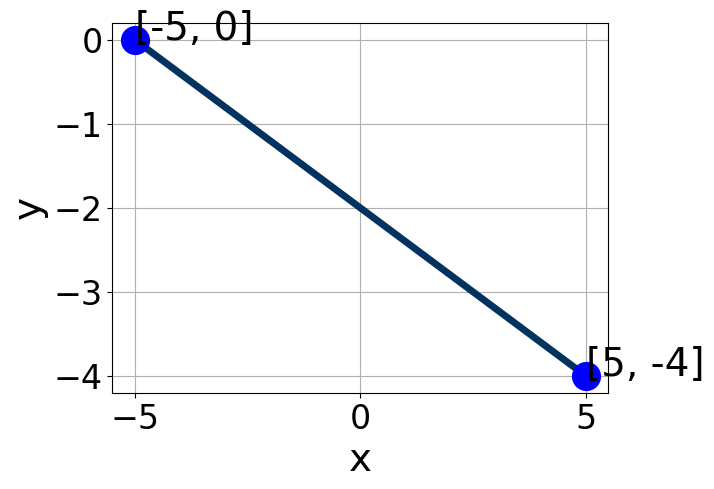
\includegraphics[width=0.5\textwidth]{../Figures/linearGraphToStandardCopyA.png}
\end{center}
\begin{enumerate}[label=\Alph*.]
\item \( A \in [-3.1, -0.3], \hspace{3mm} B \in [-7.1, -4.2], \text{ and } \hspace{3mm} C \in [8.3, 10.6] \)
\item \( A \in [-0.4, 1.1], \hspace{3mm} B \in [-2.3, -0.3], \text{ and } \hspace{3mm} C \in [0, 4.5] \)
\item \( A \in [1.6, 4.5], \hspace{3mm} B \in [3.2, 6.5], \text{ and } \hspace{3mm} C \in [-10.7, -9.3] \)
\item \( A \in [1.6, 4.5], \hspace{3mm} B \in [-7.1, -4.2], \text{ and } \hspace{3mm} C \in [8.3, 10.6] \)
\item \( A \in [-0.4, 1.1], \hspace{3mm} B \in [-0.2, 1.1], \text{ and } \hspace{3mm} C \in [-2.5, 1.1] \)

\end{enumerate} }
\litem{
Solve the linear equation below. Then, choose the interval that contains the solution.\[ \frac{8x + 5}{8} - \frac{-9x + 6}{5} = \frac{5x + 3}{2} \]\begin{enumerate}[label=\Alph*.]
\item \( x \in [11.8, 13.9] \)
\item \( x \in [-2.2, 0] \)
\item \( x \in [6.2, 7.8] \)
\item \( x \in [-0.4, 2] \)
\item \( \text{There are no real solutions.} \)

\end{enumerate} }
\litem{
Find the equation of the line described below. Write the linear equation in the form $ y=mx+b $ and choose the intervals that contain $m$ and $b$.\[ \text{Parallel to } 3 x - 5 y = 8 \text{ and passing through the point } (4, 4). \]\begin{enumerate}[label=\Alph*.]
\item \( m \in [0, 1.5] \hspace*{3mm} b \in [-0.5, 1.34] \)
\item \( m \in [1.5, 2.2] \hspace*{3mm} b \in [1.4, 2.05] \)
\item \( m \in [0, 1.5] \hspace*{3mm} b \in [1.4, 2.05] \)
\item \( m \in [-0.9, -0.2] \hspace*{3mm} b \in [6.21, 7.56] \)
\item \( m \in [0, 1.5] \hspace*{3mm} b \in [-2.12, -0.92] \)

\end{enumerate} }
\litem{
Solve the linear equation below. Then, choose the interval that contains the solution.\[ \frac{3x -9}{2} - \frac{6x + 7}{6} = \frac{-8x + 3}{7} \]\begin{enumerate}[label=\Alph*.]
\item \( x \in [1.4, 3.3] \)
\item \( x \in [0.6, 1.3] \)
\item \( x \in [2.9, 4.4] \)
\item \( x \in [11.3, 12.6] \)
\item \( \text{There are no real solutions.} \)

\end{enumerate} }
\litem{
First, find the equation of the line containing the two points below. Then, write the equation in the form $ y=mx+b $ and choose the intervals that contain $m$ and $b$.\[ (8, 3) \text{ and } (-2, -4) \]\begin{enumerate}[label=\Alph*.]
\item \( m \in [-0.48, 0.74] \hspace*{3mm} b \in [-2.85, -2.4] \)
\item \( m \in [-0.48, 0.74] \hspace*{3mm} b \in [-5.02, -4.7] \)
\item \( m \in [-0.48, 0.74] \hspace*{3mm} b \in [2.56, 3.03] \)
\item \( m \in [-0.48, 0.74] \hspace*{3mm} b \in [-2, -1.98] \)
\item \( m \in [-0.94, 0.14] \hspace*{3mm} b \in [-5.81, -5.06] \)

\end{enumerate} }
\litem{
Write the equation of the line in the graph below in Standard Form $Ax+By=C$. Then, choose the intervals that contain $A, B, \text{ and } C$.
\begin{center}
    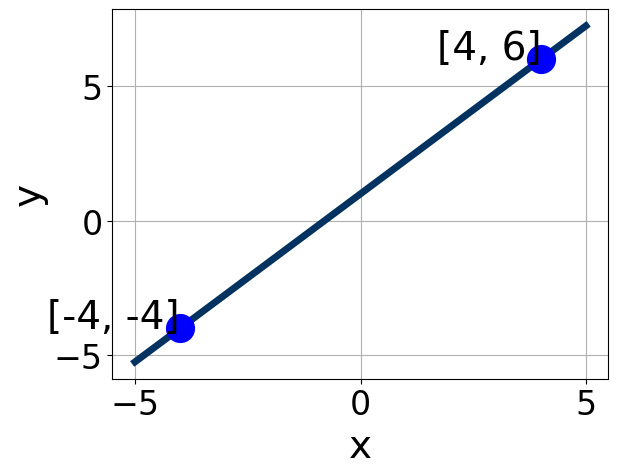
\includegraphics[width=0.5\textwidth]{../Figures/linearGraphToStandardA.png}
\end{center}
\begin{enumerate}[label=\Alph*.]
\item \( A \in [-3.25, 3.75], \hspace{3mm} B \in [-0.28, 2.73], \text{ and } \hspace{3mm} C \in [0.7, 2.5] \)
\item \( A \in [2, 9], \hspace{3mm} B \in [-4.28, -2.48], \text{ and } \hspace{3mm} C \in [-6.4, -1.6] \)
\item \( A \in [-7, -3], \hspace{3mm} B \in [2.35, 4.17], \text{ and } \hspace{3mm} C \in [3.7, 5.1] \)
\item \( A \in [-3.25, 3.75], \hspace{3mm} B \in [-2.3, -0.22], \text{ and } \hspace{3mm} C \in [-3.9, 0.4] \)
\item \( A \in [2, 9], \hspace{3mm} B \in [2.35, 4.17], \text{ and } \hspace{3mm} C \in [3.7, 5.1] \)

\end{enumerate} }
\litem{
First, find the equation of the line containing the two points below. Then, write the equation in the form $ y=mx+b $ and choose the intervals that contain $m$ and $b$.\[ (-5, 6) \text{ and } (9, 3) \]\begin{enumerate}[label=\Alph*.]
\item \( m \in [-1.7, 0.14] \hspace*{3mm} b \in [-5.04, -4.83] \)
\item \( m \in [0.16, 3.02] \hspace*{3mm} b \in [-0.09, 3.74] \)
\item \( m \in [-1.7, 0.14] \hspace*{3mm} b \in [2.8, 6.12] \)
\item \( m \in [-1.7, 0.14] \hspace*{3mm} b \in [10.9, 11.73] \)
\item \( m \in [-1.7, 0.14] \hspace*{3mm} b \in [-6.78, -5.15] \)

\end{enumerate} }
\litem{
Find the equation of the line described below. Write the linear equation in the form $ y=mx+b $ and choose the intervals that contain $m$ and $b$.\[ \text{Perpendicular to } 7 x + 8 y = 6 \text{ and passing through the point } (10, 8). \]\begin{enumerate}[label=\Alph*.]
\item \( m \in [0.99, 1.5] \hspace*{3mm} b \in [-2, 1] \)
\item \( m \in [0.06, 0.99] \hspace*{3mm} b \in [-4.43, -2.43] \)
\item \( m \in [0.99, 1.5] \hspace*{3mm} b \in [-4.43, -2.43] \)
\item \( m \in [-1.64, -0.82] \hspace*{3mm} b \in [13.43, 23.43] \)
\item \( m \in [0.99, 1.5] \hspace*{3mm} b \in [1.43, 4.43] \)

\end{enumerate} }
\litem{
Solve the equation below. Then, choose the interval that contains the solution.\[ -6(15x + 17) = -3(-19x + 18) \]\begin{enumerate}[label=\Alph*.]
\item \( x \in [-5.08, -4.19] \)
\item \( x \in [-0.63, 0.17] \)
\item \( x \in [0.24, 1.68] \)
\item \( x \in [-1.11, -0.91] \)
\item \( \text{There are no real solutions.} \)

\end{enumerate} }
\litem{
Solve the equation below. Then, choose the interval that contains the solution.\[ -11(-3x + 17) = -7(4x -14) \]\begin{enumerate}[label=\Alph*.]
\item \( x \in [-3.1, 0] \)
\item \( x \in [3.8, 6.6] \)
\item \( x \in [0.6, 2.7] \)
\item \( x \in [16.2, 18.7] \)
\item \( \text{There are no real solutions.} \)

\end{enumerate} }
\litem{
Write the equation of the line in the graph below in Standard Form $Ax+By=C$. Then, choose the intervals that contain $A, B, \text{ and } C$.
\begin{center}
    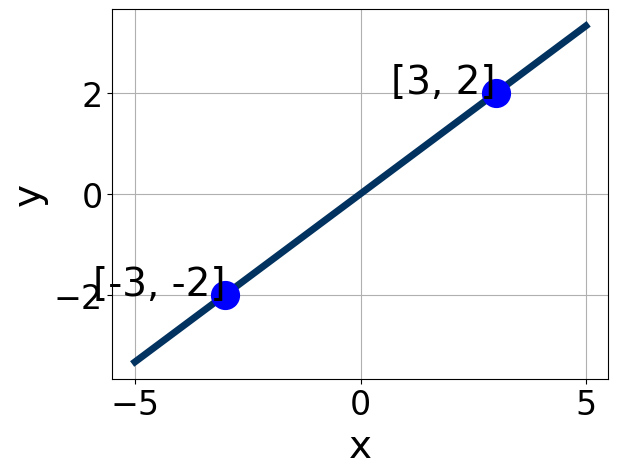
\includegraphics[width=0.5\textwidth]{../Figures/linearGraphToStandardCopyB.png}
\end{center}
\begin{enumerate}[label=\Alph*.]
\item \( A \in [-1.1, -0.5], \hspace{3mm} B \in [0.97, 1.03], \text{ and } \hspace{3mm} C \in [-1, 1] \)
\item \( A \in [-1.1, -0.5], \hspace{3mm} B \in [-2.47, -0.95], \text{ and } \hspace{3mm} C \in [-1, 1] \)
\item \( A \in [-4.3, -0.7], \hspace{3mm} B \in [1.95, 3.12], \text{ and } \hspace{3mm} C \in [-1, 1] \)
\item \( A \in [1.4, 2.8], \hspace{3mm} B \in [1.95, 3.12], \text{ and } \hspace{3mm} C \in [-1, 1] \)
\item \( A \in [1.4, 2.8], \hspace{3mm} B \in [-3.22, -1.66], \text{ and } \hspace{3mm} C \in [-1, 1] \)

\end{enumerate} }
\litem{
Solve the linear equation below. Then, choose the interval that contains the solution.\[ \frac{-9x -4}{7} - \frac{-9x -9}{5} = \frac{3x + 8}{3} \]\begin{enumerate}[label=\Alph*.]
\item \( x \in [-1.6, 0.2] \)
\item \( x \in [-3.9, -0.8] \)
\item \( x \in [-7.3, -5.8] \)
\item \( x \in [-11.5, -9.5] \)
\item \( \text{There are no real solutions.} \)

\end{enumerate} }
\litem{
Find the equation of the line described below. Write the linear equation in the form $ y=mx+b $ and choose the intervals that contain $m$ and $b$.\[ \text{Perpendicular to } 9 x - 8 y = 11 \text{ and passing through the point } (-2, -7). \]\begin{enumerate}[label=\Alph*.]
\item \( m \in [-1.2, -0.9] \hspace*{3mm} b \in [-9.45, -8.64] \)
\item \( m \in [-0.97, -0.79] \hspace*{3mm} b \in [-9.45, -8.64] \)
\item \( m \in [-0.97, -0.79] \hspace*{3mm} b \in [-5.05, -4.79] \)
\item \( m \in [-0.97, -0.79] \hspace*{3mm} b \in [8.23, 9.33] \)
\item \( m \in [0.67, 0.9] \hspace*{3mm} b \in [-5.25, -5.01] \)

\end{enumerate} }
\litem{
Solve the linear equation below. Then, choose the interval that contains the solution.\[ \frac{3x -9}{8} - \frac{-8x + 9}{5} = \frac{7x + 6}{3} \]\begin{enumerate}[label=\Alph*.]
\item \( x \in [-4.7, -1.7] \)
\item \( x \in [1.23, 4.23] \)
\item \( x \in [-14.74, -11.74] \)
\item \( x \in [-67.98, -64.98] \)
\item \( \text{There are no real solutions.} \)

\end{enumerate} }
\litem{
First, find the equation of the line containing the two points below. Then, write the equation in the form $ y=mx+b $ and choose the intervals that contain $m$ and $b$.\[ (4, 5) \text{ and } (10, -5) \]\begin{enumerate}[label=\Alph*.]
\item \( m \in [-7.67, -0.67] \hspace*{3mm} b \in [0.2, 2.9] \)
\item \( m \in [-7.67, -0.67] \hspace*{3mm} b \in [-13, -11] \)
\item \( m \in [-1.33, 5.67] \hspace*{3mm} b \in [-23.5, -18.9] \)
\item \( m \in [-7.67, -0.67] \hspace*{3mm} b \in [9.9, 13.2] \)
\item \( m \in [-7.67, -0.67] \hspace*{3mm} b \in [-16.1, -13.2] \)

\end{enumerate} }
\litem{
Write the equation of the line in the graph below in Standard Form $Ax+By=C$. Then, choose the intervals that contain $A, B, \text{ and } C$.
\begin{center}
    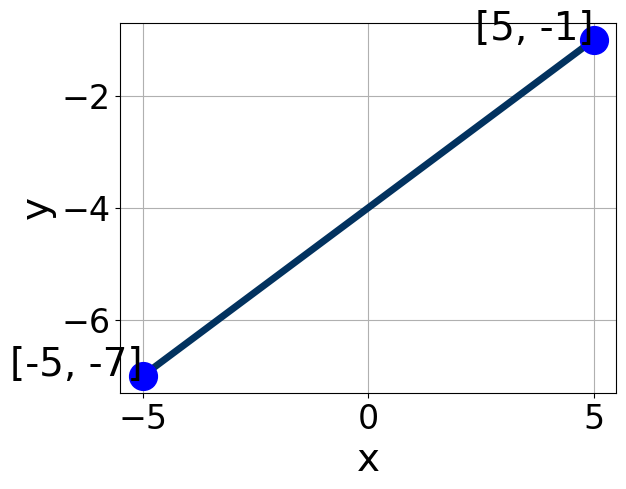
\includegraphics[width=0.5\textwidth]{../Figures/linearGraphToStandardB.png}
\end{center}
\begin{enumerate}[label=\Alph*.]
\item \( A \in [3, 12], \hspace{3mm} B \in [-7.5, -4.4], \text{ and } \hspace{3mm} C \in [20, 25] \)
\item \( A \in [-0.6, 0.4], \hspace{3mm} B \in [-3, -0.1], \text{ and } \hspace{3mm} C \in [3, 7] \)
\item \( A \in [-11, -2], \hspace{3mm} B \in [3.8, 7.8], \text{ and } \hspace{3mm} C \in [-20, -15] \)
\item \( A \in [3, 12], \hspace{3mm} B \in [3.8, 7.8], \text{ and } \hspace{3mm} C \in [-20, -15] \)
\item \( A \in [-0.6, 0.4], \hspace{3mm} B \in [-0.6, 1.4], \text{ and } \hspace{3mm} C \in [-13, 0] \)

\end{enumerate} }
\litem{
First, find the equation of the line containing the two points below. Then, write the equation in the form $ y=mx+b $ and choose the intervals that contain $m$ and $b$.\[ (9, -7) \text{ and } (-10, -3) \]\begin{enumerate}[label=\Alph*.]
\item \( m \in [-0.59, 0.04] \hspace*{3mm} b \in [6.5, 8.1] \)
\item \( m \in [-0.59, 0.04] \hspace*{3mm} b \in [4.7, 5.5] \)
\item \( m \in [-0.59, 0.04] \hspace*{3mm} b \in [-17.2, -14.8] \)
\item \( m \in [-0.59, 0.04] \hspace*{3mm} b \in [-5.5, -1.1] \)
\item \( m \in [0.07, 0.95] \hspace*{3mm} b \in [-2.3, 0.2] \)

\end{enumerate} }
\litem{
Find the equation of the line described below. Write the linear equation in the form $ y=mx+b $ and choose the intervals that contain $m$ and $b$.\[ \text{Perpendicular to } 8 x - 7 y = 9 \text{ and passing through the point } (-5, -10). \]\begin{enumerate}[label=\Alph*.]
\item \( m \in [0.58, 0.96] \hspace*{3mm} b \in [-5.8, -5.1] \)
\item \( m \in [-1.61, -1.05] \hspace*{3mm} b \in [-16.4, -11.7] \)
\item \( m \in [-0.99, -0.78] \hspace*{3mm} b \in [-5.3, -4.9] \)
\item \( m \in [-0.99, -0.78] \hspace*{3mm} b \in [11.9, 14.4] \)
\item \( m \in [-0.99, -0.78] \hspace*{3mm} b \in [-16.4, -11.7] \)

\end{enumerate} }
\litem{
Solve the equation below. Then, choose the interval that contains the solution.\[ -15(-6x + 19) = -14(12x + 4) \]\begin{enumerate}[label=\Alph*.]
\item \( x \in [-4.6, -4.26] \)
\item \( x \in [0.94, 1.57] \)
\item \( x \in [0.34, 1.31] \)
\item \( x \in [-1.67, -0.74] \)
\item \( \text{There are no real solutions.} \)

\end{enumerate} }
\litem{
Solve the equation below. Then, choose the interval that contains the solution.\[ -16(4x + 7) = -11(13x + 5) \]\begin{enumerate}[label=\Alph*.]
\item \( x \in [-1.4, 0.2] \)
\item \( x \in [1, 2.5] \)
\item \( x \in [-0.8, 1.2] \)
\item \( x \in [-2.5, -2] \)
\item \( \text{There are no real solutions.} \)

\end{enumerate} }
\litem{
Write the equation of the line in the graph below in Standard Form $Ax+By=C$. Then, choose the intervals that contain $A, B, \text{ and } C$.
\begin{center}
    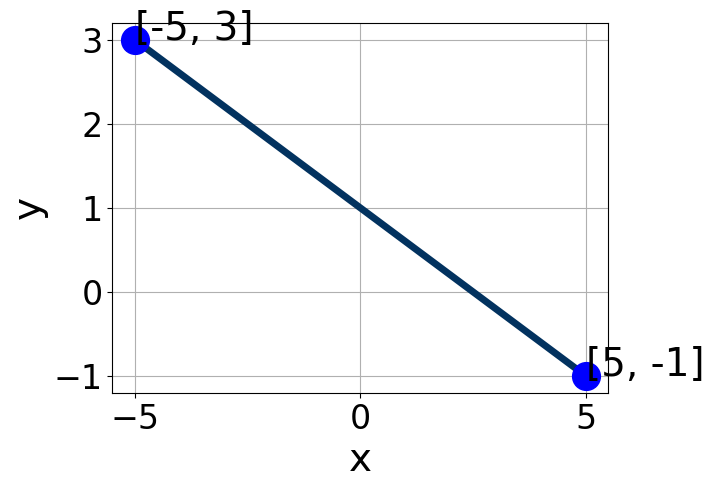
\includegraphics[width=0.5\textwidth]{../Figures/linearGraphToStandardCopyC.png}
\end{center}
\begin{enumerate}[label=\Alph*.]
\item \( A \in [-3.5, -0.3], \hspace{3mm} B \in [-6.5, -4.5], \text{ and } \hspace{3mm} C \in [-5.8, -1.4] \)
\item \( A \in [1.9, 3.7], \hspace{3mm} B \in [-6.5, -4.5], \text{ and } \hspace{3mm} C \in [-5.8, -1.4] \)
\item \( A \in [1.9, 3.7], \hspace{3mm} B \in [2.5, 6], \text{ and } \hspace{3mm} C \in [4.7, 8.4] \)
\item \( A \in [-0.4, 0.7], \hspace{3mm} B \in [0.2, 1.1], \text{ and } \hspace{3mm} C \in [-0.4, 3.2] \)
\item \( A \in [-0.4, 0.7], \hspace{3mm} B \in [-1.9, 0.5], \text{ and } \hspace{3mm} C \in [-2.4, -0.8] \)

\end{enumerate} }
\litem{
Solve the linear equation below. Then, choose the interval that contains the solution.\[ \frac{-3x -3}{2} - \frac{-7x + 6}{3} = \frac{7x -4}{8} \]\begin{enumerate}[label=\Alph*.]
\item \( x \in [-3, 1] \)
\item \( x \in [23, 29] \)
\item \( x \in [-74, -67] \)
\item \( x \in [-126, -119] \)
\item \( \text{There are no real solutions.} \)

\end{enumerate} }
\litem{
Find the equation of the line described below. Write the linear equation in the form $ y=mx+b $ and choose the intervals that contain $m$ and $b$.\[ \text{Perpendicular to } 8 x - 3 y = 7 \text{ and passing through the point } (10, -9). \]\begin{enumerate}[label=\Alph*.]
\item \( m \in [-0.16, 0.45] \hspace*{3mm} b \in [-15.75, -9.75] \)
\item \( m \in [-0.49, -0.3] \hspace*{3mm} b \in [3.25, 8.25] \)
\item \( m \in [-3.16, -2.5] \hspace*{3mm} b \in [-6.25, -1.25] \)
\item \( m \in [-0.49, -0.3] \hspace*{3mm} b \in [-21, -17] \)
\item \( m \in [-0.49, -0.3] \hspace*{3mm} b \in [-6.25, -1.25] \)

\end{enumerate} }
\litem{
Solve the linear equation below. Then, choose the interval that contains the solution.\[ \frac{-4x -9}{4} - \frac{5x -7}{6} = \frac{-5x + 8}{7} \]\begin{enumerate}[label=\Alph*.]
\item \( x \in [-1.5, 0.7] \)
\item \( x \in [-4.8, -2.6] \)
\item \( x \in [-3, -1.3] \)
\item \( x \in [-9.5, -7.7] \)
\item \( \text{There are no real solutions.} \)

\end{enumerate} }
\litem{
First, find the equation of the line containing the two points below. Then, write the equation in the form $ y=mx+b $ and choose the intervals that contain $m$ and $b$.\[ (8, 11) \text{ and } (7, -3) \]\begin{enumerate}[label=\Alph*.]
\item \( m \in [9, 15] \hspace*{3mm} b \in [3, 8] \)
\item \( m \in [9, 15] \hspace*{3mm} b \in [-10, -7] \)
\item \( m \in [-18, -9] \hspace*{3mm} b \in [94, 97] \)
\item \( m \in [9, 15] \hspace*{3mm} b \in [-101, -95] \)
\item \( m \in [9, 15] \hspace*{3mm} b \in [101, 103] \)

\end{enumerate} }
\litem{
Write the equation of the line in the graph below in Standard Form $Ax+By=C$. Then, choose the intervals that contain $A, B, \text{ and } C$.
\begin{center}
    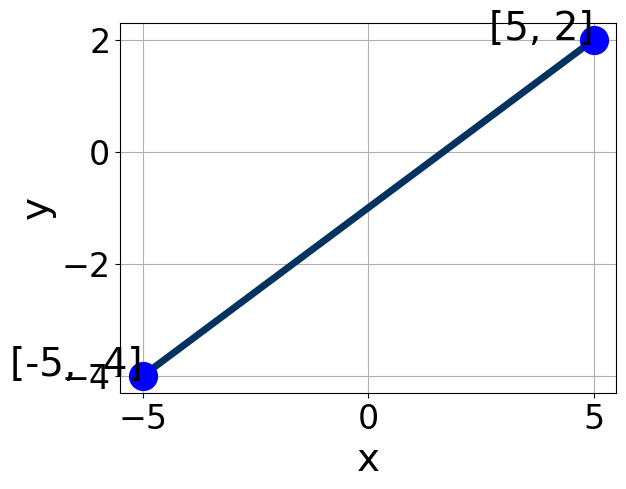
\includegraphics[width=0.5\textwidth]{../Figures/linearGraphToStandardC.png}
\end{center}
\begin{enumerate}[label=\Alph*.]
\item \( A \in [1.4, 6.1], \hspace{3mm} B \in [-5.4, -3.64], \text{ and } \hspace{3mm} C \in [3.4, 8.8] \)
\item \( A \in [-3.6, -2.4], \hspace{3mm} B \in [4.83, 5.33], \text{ and } \hspace{3mm} C \in [-7.3, -4.3] \)
\item \( A \in [-1.6, -0.5], \hspace{3mm} B \in [0.66, 1.66], \text{ and } \hspace{3mm} C \in [-2, -0.8] \)
\item \( A \in [1.4, 6.1], \hspace{3mm} B \in [4.83, 5.33], \text{ and } \hspace{3mm} C \in [-7.3, -4.3] \)
\item \( A \in [-1.6, -0.5], \hspace{3mm} B \in [-2.39, -0.89], \text{ and } \hspace{3mm} C \in [-0.7, 4.8] \)

\end{enumerate} }
\litem{
First, find the equation of the line containing the two points below. Then, write the equation in the form $ y=mx+b $ and choose the intervals that contain $m$ and $b$.\[ (-8, 11) \text{ and } (10, -5) \]\begin{enumerate}[label=\Alph*.]
\item \( m \in [0.5, 1.8] \hspace*{3mm} b \in [-14.8, -12.7] \)
\item \( m \in [-3.7, 0.5] \hspace*{3mm} b \in [1.6, 6.1] \)
\item \( m \in [-3.7, 0.5] \hspace*{3mm} b \in [-16, -14.5] \)
\item \( m \in [-3.7, 0.5] \hspace*{3mm} b \in [17.8, 21] \)
\item \( m \in [-3.7, 0.5] \hspace*{3mm} b \in [-4.4, -1.9] \)

\end{enumerate} }
\end{enumerate}

\end{document}